\documentclass[
11pt, % The default document font size, options: 10pt, 11pt, 12pt
%codirector, % Uncomment to add a codirector to the title page
]{charter} 




% El títulos de la memoria, se usa en la carátula y se puede usar el cualquier lugar del documento con el comando \ttitle
\titulo{Sistema de filtrado de agua para laboratorios} 

% Nombre del posgrado, se usa en la carátula y se puede usar el cualquier lugar del documento con el comando \degreename
\posgrado{Carrera de Especialización en Sistemas Embebidos} 

\subject{Ingeniería de Software para Sistemas Embebidos}

\versionDocument{Versión 1}
% Tu nombre, se puede usar el cualquier lugar del documento con el comando \authorname
\autor{Ing. Agustín Miguel Grosso} 

\fechaINICIO{25 de mayo de 2023}			%Fecha de inicio de la cursada de ISSE \fechaInicioName


\begin{document}

\maketitle
\thispagestyle{empty}
\pagebreak


\thispagestyle{empty}
{\setlength{\parskip}{0pt}
\tableofcontents{}
}
\pagebreak


\section*{Registros de cambios}
\label{sec:registro}


\begin{table}[H]
\label{tab:registro}
\centering
\begin{tabularx}{\linewidth}{@{}|c|X|c|@{}}
\hline
\rowcolor[HTML]{C0C0C0} 
Revisión & \multicolumn{1}{c|}{\cellcolor[HTML]{C0C0C0}Detalles de los cambios realizados} & Fecha      \\ \hline
A      	& Creación del documento                            &\fechaInicioName 		\\ \hline

\end{tabularx}
\end{table}

\pagebreak

\section{1. Introducción}
\label{sec:introduccion}
\subsection{Propósito}
\begin{enumerate}
	\item	El corriente documento desarrolla el plan de testing para el \ttitle.
	\item 	Se encuentra dirigido a la cátedra de Testing de Software Embebido de la \degreename.
\end{enumerate}

\section{2. Descripción general}
\label{sec:descripcion_general}

\subsection{Perspectiva del producto}
El software debe ser capaz de tomar mediciones y actuar en distintos periféricos incorporados en el equipo de filtrado (figura \ref{fig:microcontroladorConexiones}).
\begin{figure}[!htb]
\centering 
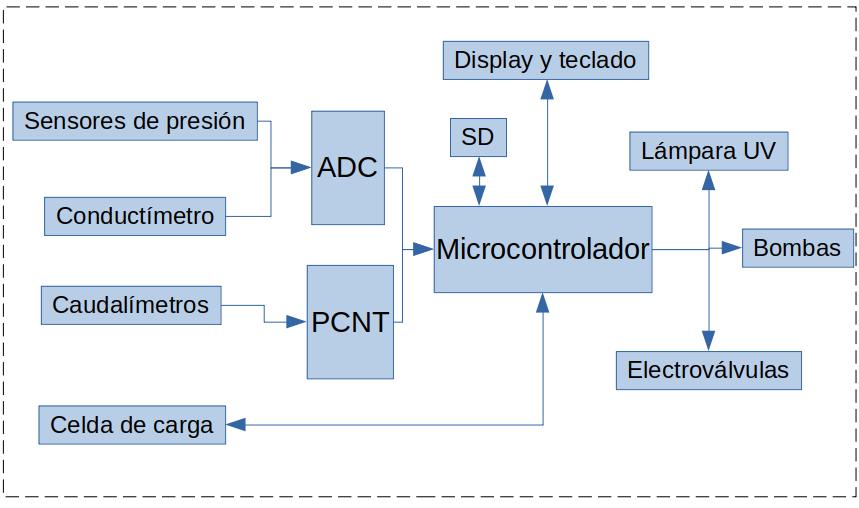
\includegraphics[width=.7\textwidth]{./Figuras/Microcontrolador y sus perifericos.png}
\caption{Microcontrolador y sus periféricos.}
\label{fig:microcontroladorConexiones}
\end{figure}

El software se integrará a un sistema diagramado con diferentes etapas (figura \ref{fig:esquemaSistema}).

\begin{enumerate}
	\item Etapa de entrada:
		\begin{itemize}
			\item Ingreso de agua al sistema.
		\end{itemize}
	\item Etapa de flush:
		\begin{itemize}
			\item Eliminación del descarte de los bloques de ósmosis.
		\end{itemize}
	\item Etapa de llenado:
		\begin{itemize}
			\item Llenado de reservorio de agua.
		\end{itemize}
	\item Lazo de filtrado:
		\begin{itemize}
			\item Re-circulación para el filtrado.
		\end{itemize}
	\item Etapa de salida:
		\begin{itemize}
			\item Erogación del agua al usuario final.
			\item Erogación del agua a segundo sistema conectado.
		\end{itemize}

\end{enumerate}


\begin{figure}[!htb]
\centering 
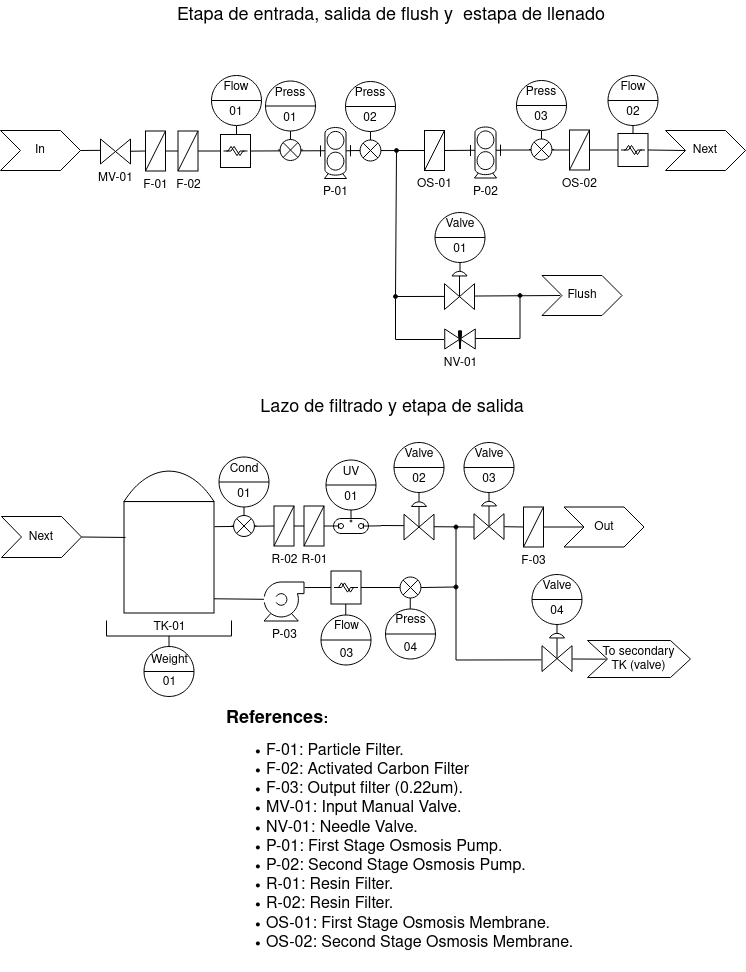
\includegraphics[width=.7\textwidth]{./Figuras/Esquema de equipo_vert.png}
\caption{Esquema del sistema de filtrado.}
\label{fig:esquemaSistema}
\end{figure}

\newpage

\subsection{Funciones del producto}
\begin{enumerate}
	\item	El software aquí descripto brindará las siguientes funcionalidades.
	\begin{enumerate}
		\item 	Control de bombas y electro-válvulas.
		\item	Gestión del almacenamiento de agua.
		\item	Control de la presión del sistema.
		\item	Control de vida útil de filtros.
		\item	Medición de conductividad.
		\item	Medición de caudal.
		\item	Medición de sólidos disueltos en agua.
		\item	Erogación de agua.
		\item	Almacenamiento de información de diagnóstico.
		\item	Presentación de información e indicaciones sobre el estado sistema.
	\end{enumerate}
	\item	El software no brindará las siguientes funcionalidades.
	\begin{enumerate}
		\item	Medición de PH, TOC, sodio, sílice, cloro.
		\item	Integración a sistema IoT.
		\item	Conexión WiFi o Bluetooth.
	\end{enumerate}
\end{enumerate}

 

\section{3. Estrategias generales}
\label{sec:estrategias_generales}
\subsection{Características de calidad}
Se realiza, a continuación, la selección de las características y subcaracterísticas de calidad seleccionadas:

\begin{itemize}
	\item \textbf{Funcionabilidad - Precisión (accurateness):} el software debe garantizar la precisión de las mediciones para lograr un correcto control de la máquina de estados que gobierna el sistema y, por lo tanto, garantizar su correcto funcionamiento. La precisión deberá cumplirse para que el resultado final sea el esperado.
	\item \textbf{Funcionabilidad - Interoperabilidad (interoperability):} el software debe tener la capacidad de detectar la necesidad de un segundo sistema de ser provisto por agua y ejecutar el proceso correspondiente para cumplir con dicha necesidad.
	\item \textbf{Utilidad - Operabilidad (operability):}  la interfaz con el usuario debe ser simple y clara para la interacción usuario-software y debe brindar información importante sobre el estado del uso del sistema.
	\item \textbf{Mantenibilidad - Analizabilidad (analyzability):} el software debe señalizar mediante salidas (leds) los estados del sistema y almacenar datos que permitan el análisis del funcionamiento actual e histórico del sistema.
	
\end{itemize}
\subsection{Importancia relativa de las características de calidad}
Se definen, en el cuadro siguiente, las características de calidad para la estrategia general de testing y su importancia relativa. 

\begin{table}[H]
\centering
\begin{tabular}{|l|c|c|}
\hline
\rowcolor[HTML]{C0C0C0}
Característica de calidad	& Subcaracterística		& Importancia relativa\\ \hline
\multirow{2}{*}{Funcionabilidad} 			& Precisión 		& 60\%	\\\cline{2-3}
  										& Interoperabilidad 	& 5\%							\\ \hline
Utilidad					& Operatividad						& 15\%						\\ \hline
Mantenibilidad				& Analizabilidad					& 20\%						\\ \hline
\end{tabular}
\caption{\centering Características de calidad del proyecto.}
\label{tab:caracteristicasDeCalidad}
\end{table}

\subsection{Características de calidad de niveles de prueba}

\begin{table}[H]
\centering
\begin{tabular}{|l|c|c|c|c|}
\hline
\rowcolor[HTML]{C0C0C0}
									& Precisión	& Interoperabilidad		& Operabilidad 	& Analizabilidad	\\ \hline
Importancia relativa				& 60 \%		& 5\%					& 15 \% 		& 20\%				\\ \hline
Unit test							& + 		&  						&  		 		& 					\\ \hline
Sotware integration test			&  			&  						&  		 		& +					\\ \hline
Hardware/software integration test	& + 		&  						&  		 		& +					\\ \hline
System test							& ++ 		& + 					& + 		 	& ++				\\ \hline
Acceptance test						& ++ 		& + 					& ++ 		 	& 					\\ \hline
Field test							& ++ 		& ++ 					& ++ 		 	& ++				\\ \hline

\end{tabular}
\caption{\centering Características de niveles de prueba.}
\label{tab:caracteristicasDeCalidadDeNivelesDePrueba}
\end{table}

Referencias:\\ \\
\begin{tabular}{l@{\hspace{2cm}}l}
\textbf{++} & La característica de calidad se cubrirá y es un objetivo principal. \\
\textbf{+} & La característica de calidad se cubrirá en este nivel de prueba. \\
\textbf{(vacío)} & La característica de calidad no es un problema en este nivel de prueba. \\
\end{tabular}

\section{4. Estrategias por nivel de prueba}
\label{sec:estrategias_nivel_de_prueba}
\subsection{Características de calidad por nivel de prueba}

\begin{itemize}
	\item Unit test	
	
		\begin{table}[H]
		\centering
		\begin{tabular}{|l|c|c|}
		\hline
		\rowcolor[HTML]{C0C0C0}
		Característica de calidad	& Subcaracterística		& Importancia relativa\\ \hline
		 Funcionabilidad 			& Precisión 		& 80\%	\\ \hline
		Mantenibilidad				& Analizabilidad					& 20\%						\\ \hline
		\end{tabular}
		\label{tab:caracteristicasDeCalidad}
		\end{table}

	\item Sotware integration test
	
	
		\begin{table}[H]
		\centering
		\begin{tabular}{|l|c|c|}
		\hline
		\rowcolor[HTML]{C0C0C0}
		Característica de calidad	& Subcaracterística		& Importancia relativa\\ \hline
		\multirow{2}{*}{Funcionabilidad} 			& Precisión 		& 25\%	\\\cline{2-3}
		  										& Interoperabilidad 	& 5\%							\\ \hline
		Utilidad					& Operatividad						& 10\%						\\ \hline
		Mantenibilidad				& Analizabilidad					& 60\%						\\ \hline
		\end{tabular}
		\label{tab:caracteristicasDeCalidad}
		\end{table}

	\item Hardware/software integration test
	
		\begin{table}[H]
		\centering
		\begin{tabular}{|l|c|c|}
		\hline
		\rowcolor[HTML]{C0C0C0}
		Característica de calidad	& Subcaracterística		& Importancia relativa\\ \hline
		\multirow{2}{*}{Funcionabilidad} 			& Precisión 		& 35\%	\\\cline{2-3}
		  										& Interoperabilidad 	& 5\%							\\ \hline
		Utilidad					& Operatividad						& 20\%						\\ \hline
		Mantenibilidad				& Analizabilidad					& 40\%						\\ \hline
		\end{tabular}
		\label{tab:caracteristicasDeCalidad}
		\end{table}

	\item System test
	
		\begin{table}[H]
		\centering
		\begin{tabular}{|l|c|c|}
		\hline
		\rowcolor[HTML]{C0C0C0}
		Característica de calidad	& Subcaracterística		& Importancia relativa\\ \hline
		\multirow{2}{*}{Funcionabilidad} 			& Precisión 		& 35\%	\\\cline{2-3}
		  										& Interoperabilidad 	& 10\%							\\ \hline
		Utilidad					& Operatividad						& 15\%						\\ \hline
		Mantenibilidad				& Analizabilidad					& 40\%						\\ \hline
		\end{tabular}
		\label{tab:caracteristicasDeCalidad}
		\end{table}

	\item Acceptance test
	
		\begin{table}[H]
		\centering
		\begin{tabular}{|l|c|c|}
		\hline
		\rowcolor[HTML]{C0C0C0}
		Característica de calidad	& Subcaracterística		& Importancia relativa\\ \hline
		\multirow{2}{*}{Funcionabilidad} 			& Precisión 		& 30\%	\\\cline{2-3}
		  										& Interoperabilidad 	& 10\%							\\ \hline
		Utilidad					& Operatividad						& 30\%						\\ \hline
		Mantenibilidad				& Analizabilidad					& 30\%						\\ \hline
		\end{tabular}
		\label{tab:caracteristicasDeCalidad}
		\end{table}

	\item Field test
	
		\begin{table}[H]
		\centering
		\begin{tabular}{|l|c|c|}
		\hline
		\rowcolor[HTML]{C0C0C0}
		Característica de calidad	& Subcaracterística		& Importancia relativa\\ \hline
		\multirow{2}{*}{Funcionabilidad} 			& Precisión 		& 35\%	\\\cline{2-3}
		  										& Interoperabilidad 	& 5\%							\\ \hline
		Utilidad					& Operatividad						& 40\%						\\ \hline
		Mantenibilidad				& Analizabilidad					& 20\%						\\ \hline
		\end{tabular}
		\label{tab:caracteristicasDeCalidad}
		\end{table}

\end{itemize}

\subsection{División del sistema en subsistemas}
Se definen, para el \ttitle, los siguientes subsistemas.
\begin{enumerate}
        \item \textbf{Subsistema A: Subsistema de adquisición}\\
        Adquisición de datos provenientes de sensores, pulsadores y datos internos(caudal, conductividad, presión, volumen en reservorio, pulsadores, tiempo de funcionamiento).
        \item \textbf{Subsistema B: Subsistema de análisis y control}\\
        Análisis de los datos adquiridos por el subsistema de adquisición y determinación de estado siguiente del sistema.
        \item \textbf{Subsistema C: Subsistema de actuación}\\
        Actuación sobre bombas, lámpara UV, electro-válvulas en base al estado del sistema definido por el subsistema de análisis y control.
        \item \textbf{Subsistema D: Subsistema de almacenamiento de datos}\\
        Almacenamiento en memoria SD de los datos recibidos del subsistema de análisis y control.
        \item \textbf{Subsistema E: Subsistema de display}\\
        Informe de estado del sistema y mensajes hacia el usuario.
\end{enumerate}

\subsection{Importancia relativa de los subsistemas}


\begin{table}[H]
\centering
\begin{tabular}{|l|c|c|}
\hline
\rowcolor[HTML]{C0C0C0}
Subsistema 							& Importancia relativa\\ \hline
Subsistema de adquisición								& 25\%						\\ \hline
Subsistema de análisis y control						& 25\%						\\ \hline
Subsistema de actuación									& 25\%						\\ \hline
Subsistema de almacenamiento de datos					& 10\%						\\ \hline
Subsistema de display									& 15\%						\\ \hline
\end{tabular}
\caption{\centering Subsistemas y su importancia relativa.}
\label{tab:subsistemas_importancia}
\end{table}

\subsection{Determinación de la importancia de test por combinaciones de subsistema y características de calidad}
\begin{table}[H]
\centering
\begin{tabular}{|l|c|c|c|c|c|}
\hline
\rowcolor[HTML]{C0C0C0}
& Sub. A & Sub. B & Sub. C & Sub. D & Sub. E    \\ \hline
\rowcolor[HTML]{EFEFEF}
Importancia relativa					& 25\% & 25\% & 25\% & 10\% & 15\%						\\ \hline
Precisión								& ++ & ++ 	& ++ 	& + 	& 					\\ \hline
Interoperabilidad						&  + & + 	& + 	&  		& 						\\ \hline
Operabilidad							&  + &+  	& + 		&  		& ++						\\ \hline
Analizabilidad					 		& +  & + 	& + 	& ++ 	& ++				\\ \hline
\end{tabular}
\caption{\centering Características de calidad por subsistema.}
\label{tab:subsistemas_importancia}
\end{table}


Referencias:\\ \\
\begin{tabular}{l@{\hspace{2cm}}l}
\textbf{++} & La característica de calidad se cubrirá y es un objetivo principal. \\
\textbf{+} & La característica de calidad se cubrirá en este nivel de prueba. \\
\textbf{(vacío)} & La característica de calidad no es un problema en este nivel de prueba. \\
\end{tabular}

\subsection{Técnicas de test a ser usadas}
Se determinan las técnicas de test a usar sobre el software:
\begin{itemize}
	\item STT (State Transition Testing)\\
	Test aplicable a la máquina de estados desarrollada con FreeRTOS.
	\item CFT (Control Flow Testing)\\
	Test aplicable a caminos determinados dentro del software desarrollados.
	\item ECT (Elementary Comparison Testing)\\
	Test aplicable a las mediciones obtenidas por los sensores y a las decisiones tomadas a partir de los valores medidos.
\end{itemize}
\end{document}
